\setlength{\resLen}{.47\columnwidth}
\begin{figure}[t]
	\addtolength{\tabcolsep}{-4pt}
	\begin{tabular}{c @{\hspace{2\tabcolsep}} ccc}
	\raisebox{.15in}{\rotatebox[origin=c]{90}{\footnotesize{GT}}} &
	\includegraphics[width=\resLen]{validation/embed/fake_018/tex_ref.jpg} & &
	\includegraphics[width=\resLen]{validation/embed/fake_037/tex_ref.jpg}
	\\
	\raisebox{.15in}{\rotatebox[origin=c]{90}{\footnotesize{$\calW$}}} & 
	\includegraphics[width=\resLen]{validation/embed/fake_018/tex_W.jpg} & &
	\includegraphics[width=\resLen]{validation/embed/fake_037/tex_W.jpg}
	\\
	\raisebox{.15in}{\rotatebox[origin=c]{90}{\footnotesize{$\calW^+$}}} &
	\includegraphics[width=\resLen]{validation/embed/fake_018/tex_W+.jpg} & &
	\includegraphics[width=\resLen]{validation/embed/fake_037/tex_W+.jpg}
	\\
	\raisebox{.15in}{\rotatebox[origin=c]{90}{\footnotesize{$\calW^+\calN$}}} &
	\includegraphics[width=\resLen]{validation/embed/fake_018/tex_W+N.jpg} & &
	\includegraphics[width=\resLen]{validation/embed/fake_037/tex_W+N.jpg}
	\end{tabular}
	\caption{\label{fig:embed}
		\textbf{Embedding SVBRDFs into different latent spaces.} We take two synthetic SVBRDF material maps (top) and embed them into different latent spaces with and without the noise space (second--fourth rows). For illustration, we also embed the maps into a pure-noise space \emph{only}; this is unable to recover the color at all.
	}
\end{figure}